\Chapter{Beam Line Design}%________________________________
\Section{Kicker Design}

\lsnote{You need to start with a re-statement of the purpose of the kicker. }
A design implemented by Indiana University (IU) \cite{iukicker}
will be adapted to fit TBA requirements at the AWA. Redesign will require optimization
of the length and gap between the kicker plates. \lsnote{Summarize what criteria are used to determine these.} Figure \ref{fig:IUkicker} shows the existing IU kicker.
\begin{figure}[h]
	\begin{center}
		%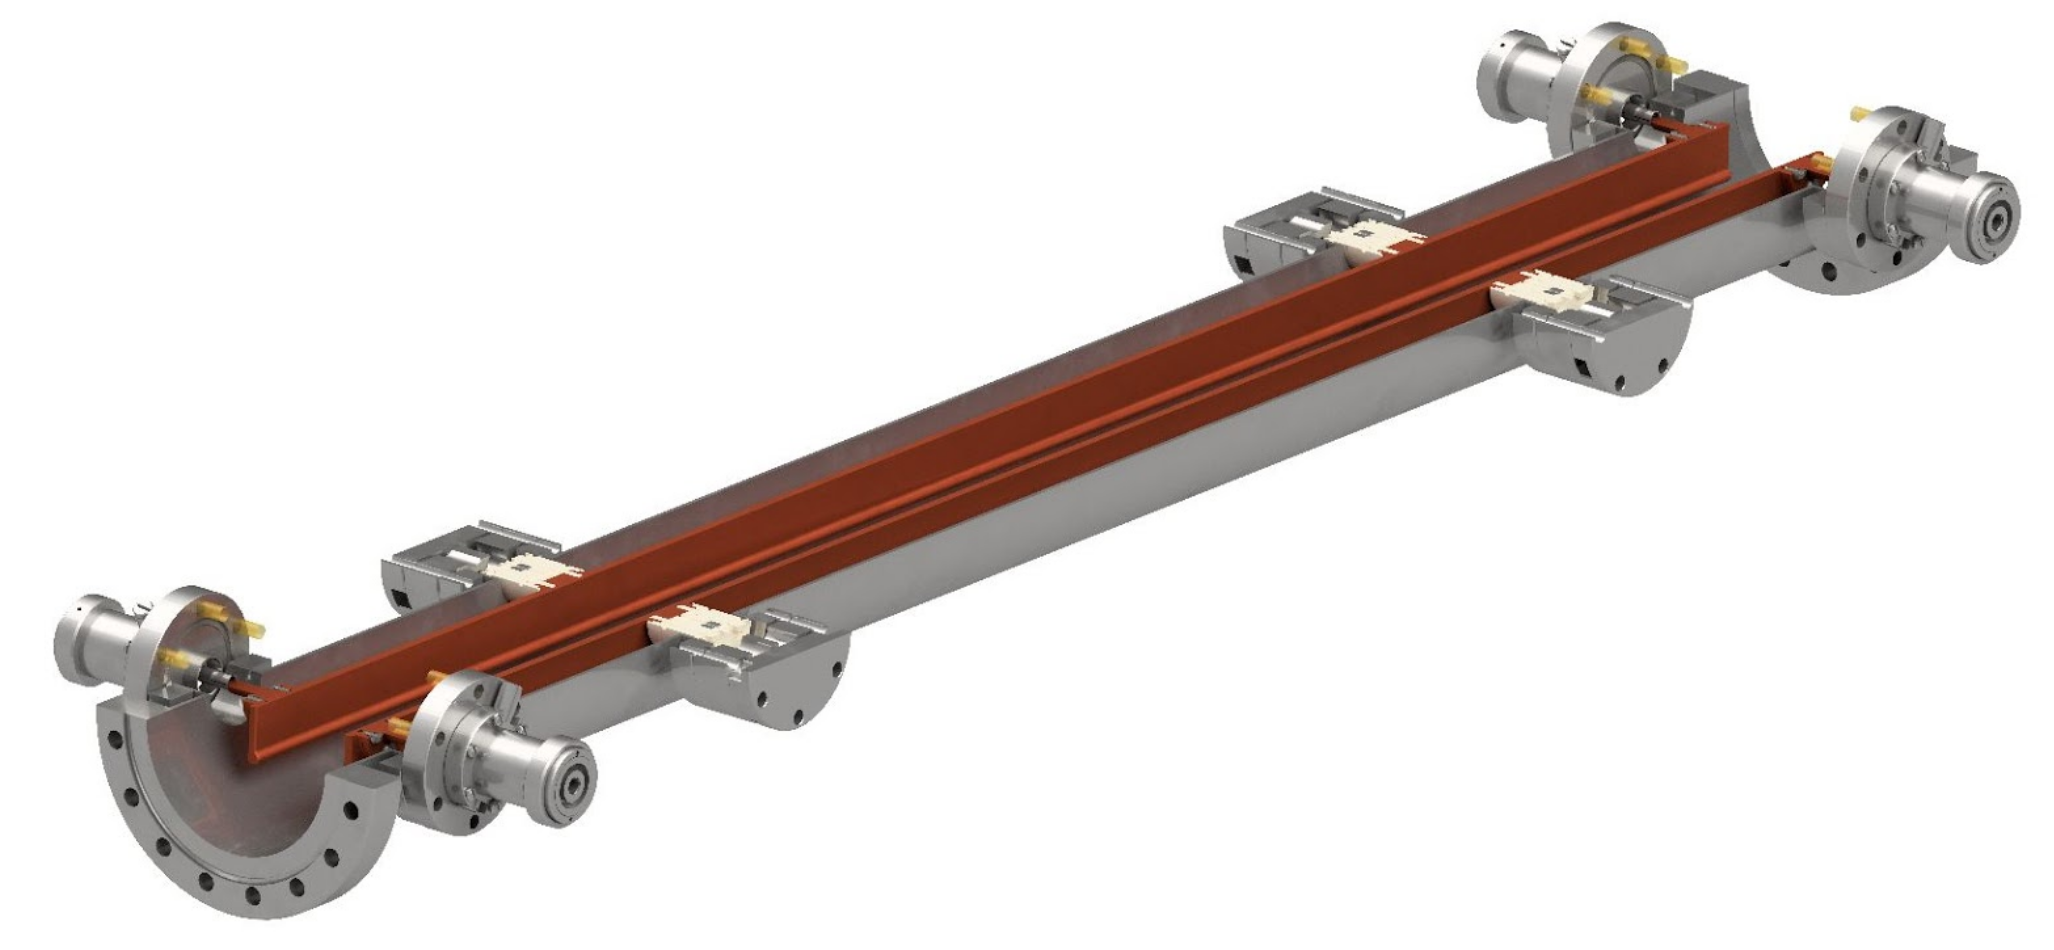
\includegraphics[scale=0.5]{C:/Users/nneveu/Pictures/kicker.jpg}\caption{IU Kicker \cite{IUkicker}}
		\label{fig:IUkicker}
	\end{center}
\end{figure}
The kicker is essentially a parallel plate waveguide. 
A $\pm$35 kV power supply will be used to induce a 70 kV potential difference 
across the plates. Each plate will be terminated in a 50 $\Omega$ load to induce a steady 
state current on the plates. The combination of the two will result in a static TEM mode 
between the plates. Calculation of the electric, $E_v$, and magnetic field, $B_v$,
can be derived from the voltage or current. The electric field, $E_v$, due to a potential, V, is: 
\begin{equation}
E_v=\frac{V}{h}
\end{equation}

Where h is the gap height. From Maxwell's equations, we know that the electric and magnetic 
field are related by the speed of light, c, in the case of plane and TEM waves \cite{pozar}. 
From this we can find the magnetic field induced between the plates: 
\begin{equation}
B_v=\frac{E_v}{c}
\end{equation}
The electrons are going at the speed of light, $c$, and are moving through the kicker on a 
trajectory perpendicular to the fields.  So, it can be seen from the Lorentz force equation, that the force 
exerted on a charge q from the electric and magnetic fields of the TEM mode are equal. 
\begin{equation}
F=q(E_v+v\times B_v)
\end{equation}

Since the force due to the electric field is equal and in the same direction as that from the magnetic field, 
the total kick is just twice that from either field alone.  The angle induced by each field is \cite{iukicker, Wiedemann}:  
\begin{equation}
\theta_E= \frac{V\,L}{h\,T}
\end{equation}
\begin{equation}
\theta_B= \frac{B\,L}{B\rho}
\end{equation}

Where L is the plate length, and T is the kinetic energy of the beam. $B\rho=3.33564\,*T\,$ [GeV-Tesla] is a 
common accelerator physics term that can be found in text such as Wiedemann \cite{Wiedemann}. 
The total angle provided by the kicker is then: 
\begin{equation}
\theta_{total}= \theta_E+\theta_B=2\theta_E=2\theta_B
\end{equation}
From these equations, variable parameters include the gap height, length of the plates, and 
the kinetic energy of the beam. The largest drive beam energy achievable at the AWA is 75 MeV. 
Thesis work will include the optimi
zation of these parameters to obtain the largest angle possible.
Simulations have begun to set boundary conditions on the variable parameters. 





Using the foundations set in Chapters 2 and 3, 
\nrnote{Change foundations to more elaborate description...
beam line requirements, diagnostics at AWA, etc...???}
a beam line design for staged 
two beam acceleration was laid out and simulated. 
\nrnote{.....more intro here...do I need to spell out building block matrices?}

A drift: 
\begin{equation}
R_d = 
\begin{bmatrix}
1 & L \\
0 & 1
\end{bmatrix}
\end{equation}

A quad: 
\begin{equation}
R_q = 
\begin{bmatrix}
1 & 0 \\
\pm \frac{1}{f} & 1
\end{bmatrix}
\end{equation}

A dipole:
\begin{equation}
R_s = 
\begin{bmatrix}
0 & 0 \\
0 & 0
\end{bmatrix}
\end{equation}

To convert from focal length to quadrupole strength we must take into account the 
beam energy as well as the dimensions of the quadrupole. 
\begin{equation}
	\frac{1}{f} = kl \\
\end{equation}
Where $l$ is the quadrupole's effective length, and k is the gradient w.r.t 
the beam energy and magnet strength \cite{Wiedemann}:
\begin{equation}
	k = \SI{0.2998}{} \frac{g[\SI{}{T/m}]}{p [\SI{}{GeV/c}]}\label{k}
\end{equation}

\Section{Matrix Formalism For TBA Beam Line}

 To reduce the number of free parameters quickly without using expensive PIC simulations, 
 the transfer matrix of the beam line was considered. Starting at the end of the linac, 
 we consider the first four quadrupoles before the kicker. All the quadruple strengths (4) and
 distances between the quadrupoles (6) are parameters under consideration. To reduce the number
 of variables from 10 to 4, we use the quadruplet telescope module as described by K. Brown in \cite{brown}.  The transfer matrix R, is reduced to:  
 \begin{equation}
 R_q = R_{d4} \cdot R_{q3} \cdot R_{d3} \cdot R_{q2} \cdot R_{d2} \cdot R_{q1} \cdot R_{d1} = 
 \begin{bmatrix}
 \frac{f_2 f_4}{f_1 f_3} & 0 \\
 0 & \frac{f_1 f_3}{f_2 f_4}	
 \end{bmatrix}\label{kb1}
 \end{equation}

\nrnote{add detail about this matrix comes from and expand matrix to x and y}
Where $f_1 \ldots f_4$ stand for the focal lengths of each quad before the kicker. 
Due to other experiments in the AWA tunnel, 
the first quadrupole was required to be at least $\SI{3}{m}$ away from the exit of the 
last accelerating cavity in the linac. This gives the initial drift length and value
for $f_1$. 

\Subsection{Point to Point Configuration}
To achieve point to point transport of the beam, we can 
equate $f_1 = f_4$ and $f_2 = f_3$. This reduces Eq. \ref{kb1} to:
 \begin{equation}
R_q =
\begin{bmatrix}
1 & 0 \\
0 & 1	
\end{bmatrix}
\end{equation}
We can further simplify the experimental set up by 
assuming $f_1=f_2$. Given the total distance, D, available for the
quads in the beam line, \SI{3.8}{m}, we can then solve
for the focal length $f_1$: 
\begin{align}
	D = 4f_1 + 4 f_2 = 8f_1 = \SI{3.8}{m} \\
	f_1 = \SI{0.475}{m}
\end{align}
Given an energy of \SI{65}{MeV}, a quadrupole length of \SI{11}{cm}, 
and Eq. \ref{k} we can calculate this configuration would require a 
magnet strength of \SI{4.14}{[T/m]}. This is feasible considering the 
max strength is \SI{9}{[T/m]}.

To determine the effect of this configuration on the beam size and divergence
we compare the sigma matrix before and after the qudrupoles:
\begin{align}
	\sigma_1 = R\cdot \sigma_0 \cdot R^T \\
	= 
	\begin{bmatrix}
	1 & 0 \\
	0 & 1	
	\end{bmatrix}
	\begin{bmatrix}
	1 & 0 \\
	0 & 1	
	\end{bmatrix}
    \begin{bmatrix}
	1 & 0 \\
	0 & 1	
	\end{bmatrix} \\
	=
	\begin{bmatrix}
	1 & 0 \\
	0 & 1	
	\end{bmatrix}
\end{align}

\Subsection{Point to Parallel Configuration}
Having less divergence entering the kicker may be more beneficial than 
maintaining the initial beam distribution. 

\iffalse 
 \[
 \begin{bmatrix}
 x_{11}       & x_{12} & x_{13} & \dots & x_{1n} \\
 x_{21}       & x_{22} & x_{23} & \dots & x_{2n} \\
 \hdotsfor{5} \\
 x_{d1}       & x_{d2} & x_{d3} & \dots & x_{dn}
 \end{bmatrix}
 =
 \begin{bmatrix}
 x_{11} & x_{12} & x_{13} & \dots  & x_{1n} \\
 x_{21} & x_{22} & x_{23} & \dots  & x_{2n} \\
 \vdots & \vdots & \vdots & \ddots & \vdots \\
 x_{d1} & x_{d2} & x_{d3} & \dots  & x_{dn}
 \end{bmatrix}
 \]
 \fi